%!TEX root = ../report.tex
\chapter{Background Theory}
%OR: \chapter{Tools and Methods}
\label{cha:background_theory}

\section{Definitions}
\begin{description}
    \item[Result tree:] {\em Result r for a given query q with tokens Qt on an RDF graph G$\langle$V, E$\rangle$, where the result forms a minimum spanning tree Tm$\langle$V', E'$\rangle$, V' contains a set of tokens Tt, Tm is rooted in a place vertex p, so that V' $\subseteq$V, E'$\subseteq$E, and Tt$\subseteq$Qt}
\end{description}
All results from a query is given as a minimum spanning tree. This tree is call a {\em Result Tree}. A query can have multiple result trees, where each result tree is rooted in a unique place node, and each tree contains at least one query word.

\begin{description}
    \item[Root:] {\em Any GeoEntity node used as a start when traversing the graph, and as the place node in a result tree}
\end{description}

\begin{description}
    \item[Accuracy:] {\em Score given to a result tree, where score is based on the number of nodes n in the result tree, node distance nd from root, query q, and number of query words hit h so that $\mathcal{F}_h = (h_i/\left\lvert q \right\rvert : i \in \mathcal{I})$ and $ \frac{\sum \mathcal{F}_h}{n*(nd+1)}$}
\end{description}


Knowledge base, ontology and knowledge graph are terms with multiple definitions, and are often used interchangeably. The definitions here are used to clarify what they mean in this paper, and is not a definitive definition.

\subsection{Knowledge Base}
The term knowledge base can have many definitions, often because the terms knowledge base, ontology, and knowledge graph is used interchangeably \citep{KGDef}. In this paper the term knowledge graph will be defined as follows: ``A knowledge base is a data set with some formal semantics. This could include multiple axioms, definitions, rules, facts, statements, and other primitives.'' \citep{davies2006semantic}

\subsection{Ontology}
Like knowledge base, ontology does not have one clear definition. This is because the term have many different interpretations, and is often confused with other terms \citep{FEILMAYR20161}. Most definitions of ontologies say that ontologies represent a schema, basic theory, or conceptualization of a domain, which knowledge bases do not. \citep{davies2006semantic} To differentiate ontologies and knowledge bases in this paper the definition of an ontology will be ``An ontology is an extended knowledge base that allows for semantic modeling of knowledge.'' With this definition, ontologies can be considered a specialized form of knowledge bases.

\subsection{Knowledge Graphs}
A broad definition of knowledge graph is ``A knowledge graph acquires and integrates information into an ontology and applies a reasoner to derive new knowledge.'' \citep{KGDef} This definition is encompasses multiple technologies. In this paper we will use the more specific definition that fits the data used ``We define a Knowledge Graph as an RDF graph. An RDF graph consists of a set of RDF triples where each RDF triple (s, p, o) is an ordered set of the following RDF terms: a subject s $\in$ U $\cup$ B, a predicate p $\in$ U, and an object U $\cup$ B  L. An RDF term is either a URI u $\in$ U, a blank node b $\in$ B, or a literal l $\in$ L'' \citep{KGDefYago}

\subsubsection{Subject}
In a RDF triple the subject is a URI or a blank node. The URI when used in the subject identifies an entity, or is an alias, different language or other variation of an entity. This subject can have relations to objects describing the same entity.

\subsubsection{Predicate}
Predicates are always a URI. URIs used for predicates differ from the ones used for subjects and objects in that predicates are of a type. A type is an identifier used to describe the relation between the subject and object.

\subsubsection{Object}
Objects have the widest range of possible entries. Like subjects and predicates, objects can be URIs. Object URIs can be entity identifiers like subjects, they can be class identifiers, or they can contain some data and a data type. Blank nodes are just that, blank, and literals are an atomic value. 

\subsection{Facts and entities}
A fact is a term often used when describing knowledge bases, ontologies and knowledge graphs. Usually a fact is the smallest piece of information in such a system. In a knowledge graph this is a single RFD triple. Another term often used is entity. An entity is a collection of facts, usually from the same article. Entities can be linked together through facts. In such a fact, one entity is used as the subject, the predicate describes the relation, and the object is the other entity. In such a relation both entities will be URIs.



\section{Existing knowledge graphs and ontologies}
Currently two of the largest open technologies for knowledge graphs are Yago and DBPedia. Both these projects use automatic extraction from Wikipedia to create the graph, but differ in the ontology used to build the graphs. Yago also includes data from WordNet and GeoNames to accurately assign entities to classes. Both projects use RDF triples to create a knowledge graph.\\
% When a set of articles are linked they form a graph with each article being a entity in this graph\cite{mahdisoltani:hal-01699874, hoffart2013yago2}. Most articles falls into one or more categories, which is in turn used create a taxonomy of the entities. Since a category can be a subset of a different category, this creates a hierarchy of different entities based on what categories an entity falls under. Using the entity and category, combined with the linking of articles it is possible to create a directed graph of entities.

% - How can a knowledge base be described as a graph\\
% Knowledge graphs is usually structured with a subject, predicate, and object. Both the subject and object are entities, or facts, and the predicate describes the relation between two facts. This structure makes the graph a directed cyclic graph. An example of the subject predicate object can be "Nidaros Cathedral" "is located in" "Trondheim".\\

% - Graphic depicting some KG.\\
\subsection{Uses for Knowledge graphs}
One of the uses of knowledge graphs today is to find and display a info box in search engines. This information is a compact set of facts that tries to fit the search query. Because of the graph structure of knowledge graphs the information in the info box can be adapted to the query by choosing the predicates and related facts closest related to the query. This makes it possible to create a set of information that can give the user a quick overview of the information retrieved by the query.

\subsection{Yago}
Yago is an acronym for Yet Another Great Ontology, and is main data source in this paper. The project describes it self as a knowledge base\citep{yago} and an ontology \citep{mahdisoltani:hal-01699874}, but is often described as a knowledge graph by others. In this paper Yago is described as a knowledge graph.

\subsubsection{Temporal data}
Yago have many entities with facts describing date and spatial data.\citep{yago} Date facts follows the ISO 8601 format, YYYY-MM-DD, and introduces \# as a wildcard symbol. A fact can only hold information on a single point in time, and uses yagoDate as a data type in addition to information on the date.\citep{yago} In a date fact, the object holds the date information, and the predicate describes a connection between subject and date. ``Nidaros\_Cathedral wasCreatedOnDate 1300-\#\#-\#\# .'' In this example the predicate wasCreatedOn is used to describe a relation between the subject and a date.

To describe a time span two facts are required. One of the facts describes a start date, and the second en end date. Since an entity can have multiple date facts connected, all date predicates are also assigned to a class. Start dates are assigned to a predicate with a type that has a ``creation'' class, such as ``StartedOnDate''. End dates are assigned to ``destruction'' type predicates. This makes it possible to deduce a time span for a given subject and predicate combination.\citep{yago}

\subsubsection{Spatial data}
Yago only contains permanent spatial data for entities on earth. This means that entities like cities, buildings, rivers and mountains are given a spatial dimension. In addition, events, people, groups and artifacts can be given a spatial dimension by relating the entity to a specific place. All spatial facts must have a predicate that fall under the yagoGeoEntity class, and all objects used in a fact with a yagoGeoEntity must have a relation containing both ``hasLatitude'' and ``hasLongitude''.

\subsection{DBPedia}

\subsection{Jena}
Apache Jena is a set of tools for working with RDF and other semantic web, and linked data. The framework contains tools for querying with SPARQL, a query language made specifically for RDF graphs. Jena also contains REST-style SPARQL endpoints making the RDF data easily accessible. Using the existing standards makes it easy to use existing data sets, such as Yago or DBPedia, and build utility on top of that data using some of the tools Jena provides.


\section{Introducing Figures}
\begin{figure}[t]
  \centering
  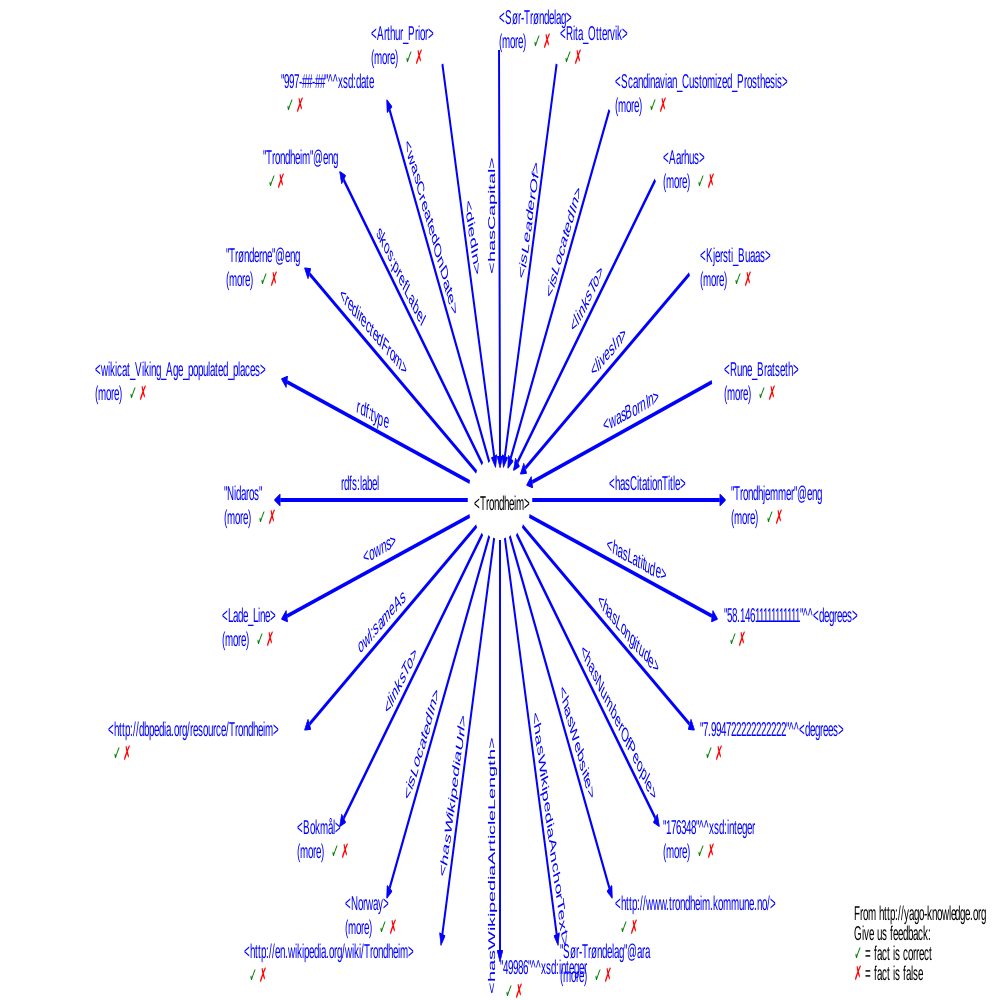
\includegraphics[scale=0.3]{figs/yago_trondheim.png}
 \caption{Trondheim as a subject in YAGO}
 \label{fig:Trondheim}
\end{figure}

\begin{figure}[t]
  \centering
  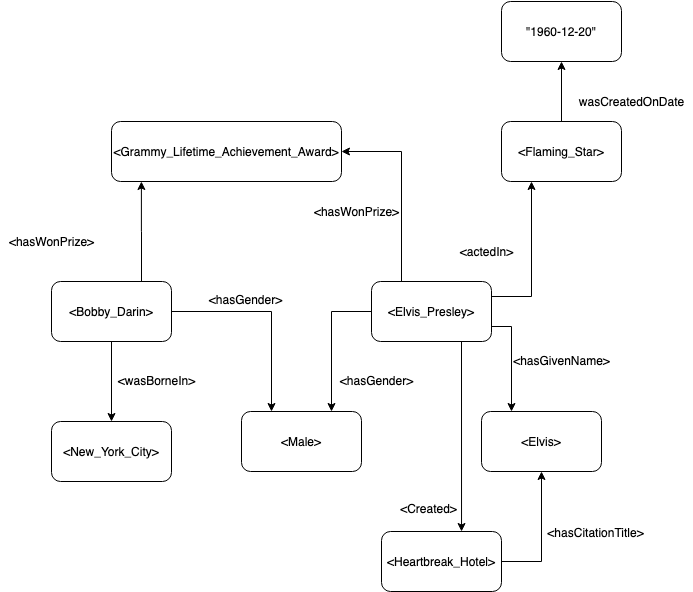
\includegraphics[scale=0.5]{figs/yagoExample.png}
 \caption{Connections in Yago around Elvis}
 \label{fig:Elvis}
\end{figure}

\section{Introducing Tables in the Report}

\glsresetall
